\documentclass[11pt]{article}
\usepackage[utf8]{inputenc} 
\usepackage[T1]{fontenc}    
\usepackage{url}            
\usepackage{booktabs}       
\usepackage{amsfonts}       
\usepackage{nicefrac}
\usepackage{microtype}      
\usepackage{fullpage}
\usepackage{subcaption}
\usepackage[most]{tcolorbox}
\usepackage[numbers]{natbib}
%\usepackage[textsize=tiny]{todonotes}
\setlength{\marginparwidth}{11ex}

\newcommand{\E}{\mathbb E}
\usepackage{wrapfig}
\usepackage{caption}

\newcommand{\theHalgorithm}{\arabic{algorithm}}

\usepackage{url}

\usepackage[utf8]{inputenc}
\usepackage{amsmath}
\usepackage{graphicx}
\usepackage{upgreek}
\usepackage{amsfonts}
\usepackage{amssymb}
\usepackage{amsthm}
\usepackage[mathscr]{euscript}
\usepackage{mathtools}
\newtheorem{thm}{Theorem}
\newtheorem{defn}{Definition}
\newtheorem{cor}{Corollary}
\newtheorem{assumption}{Assumption}
\newtheorem{lem}{Lemma}
\usepackage{xcolor}
\usepackage{nicefrac}
\usepackage{xr}
%\usepackage{chngcntr}
\usepackage{apptools}
\usepackage[page, header]{appendix}
\AtAppendix{\counterwithin{lem}{section}}
\usepackage{titletoc}
\usepackage{enumitem}
\setlist[itemize]{leftmargin=1cm}
\setlist[enumerate]{leftmargin=1cm}
\newcommand*{\fnref}[1]{\textsuperscript{\ref{#1}}}



\definecolor{DarkRed}{rgb}{0.75,0,0}
\definecolor{DarkGreen}{rgb}{0,0.5,0}
\definecolor{DarkPurple}{rgb}{0.5,0,0.5}
\definecolor{Dark}{rgb}{0.5,0.5,0}
\definecolor{DarkBlue}{rgb}{0,0,0.7}
\usepackage[bookmarks, colorlinks=true, plainpages = false, citecolor = DarkBlue, urlcolor = blue, filecolor = black, linkcolor =DarkGreen]{hyperref}
\usepackage{breakurl}
\usepackage[ruled, vlined, linesnumbered]{algorithm2e}
\newcommand\mycommfont[1]{\footnotesize\ttfamily\textcolor{blue}{#1}}
\SetCommentSty{mycommfont}

\DeclareMathOperator*{\argmin}{arg\,min}
\DeclareMathOperator*{\argmax}{arg\,max}

\allowdisplaybreaks[2]
\newcommand{\prob}{\mathbb P}
\newcommand{\Var}{\mathbb V}
\newcommand{\NN}{\mathbb N}
\newcommand{\Ex}{\mathbb E}
\newcommand{\varV}{\mathscr V}
\newcommand{\indicator}[1]{\mathbb I\{ #1 \} }
\newcommand{\statespace}{\mathcal S}
\newcommand{\actionspace}{\mathcal A}
\newcommand{\saspace}{\statespace \times \actionspace}
\newcommand{\satspace}{\mathcal Z}
\newcommand{\numsa}{\left|\saspace\right|}
\newcommand{\numsat}{\left|\satspace\right|}
\newcommand{\numS}{S}
\newcommand{\numA}{A}
\newcommand{\wmin}{w_{\min}}
\newcommand{\wminc}{w'_{\min}}
\newcommand{\range}{\operatorname{rng}}
\newcommand{\polylog}{\operatorname{polylog}}
\newcommand{\dspace}{\mathcal D}
\newcommand{\numD}{|\dspace|}
\newcommand{\numSucc}[1]{|\statespace(#1)|}
\newcommand{\succS}[1]{\statespace(#1)}

\newcommand{\reals}{\mathbb R}
\newcommand{\const}{\textrm{const.}}
\newcommand{\set}[1]{\left\{#1\right\}}
\newcommand{\llnp}{\operatorname{llnp}}
\newcommand{\defeq}{:=}
\usepackage{xspace}
\newcommand{\algname}{UBEV\xspace}

\mathtoolsset{showonlyrefs=true}

\let\temp\epsilon
\let\epsilon\varepsilon
\newcommand{\cK}{\mathcal K}
\newcommand{\cI}{\mathcal I}
\newcommand{\Pro}{\mathbb P}

\title{CS 234 Spring 2024 \\ Assignment 1 \\ Due: April 12 at 6:00 pm (PST)}
\date{}

\begin{document}
  \maketitle
\noindent For submission instructions, please refer to the \href{http://web.stanford.edu/class/cs234/assignments.html}{website}.
For all problems, if you use an existing result from either the literature or a textbook to solve the exercise, you need to cite the source.


\section{Effect of Effective Horizon [8 pts]} 

Consider an agent managing inventory for a store, which is represented as an MDP. The stock level $s$ refers to the number of items currently in stock (between 0 and 10, inclusive). At any time, the agent has two actions: sell (decrease stock by one, if possible) or buy (increase stock by one, if possible).  
\begin{itemize}
\item If $s 
 > 0$ and the agent sells, it receives +1 reward for the sale and the stock level transitions to $s - 1$. If $s = 0$ nothing happens.
 \item If $s < 9$ and the agent buys, it receives no reward and the stock level transitions to $s +  1$.
 \item The owner of the store likes to see a fully stocked inventory at the end of the day, so the agent is rewarded with $+100$ if the stock level ever reaches the maximum level $s = 10$.
 \item $s = 10$ is also a terminal state and the problem ends if it is reached.
\end{itemize}

The reward function, denoted as $r(s, a, s')$, can be summarized concisely as follows:
\begin{itemize}
    \item $r(s,\text{sell}, s-1) = 1$ for $s > 0$ and $r(0,\text{sell},0) = 0$
    \item $r(s, \text{buy}, s+1) = 0$ for $s < 9$ and $r(9, \text{buy}, 10) = 100$. The last condition indicates that transitioning from $s = 9$ to $s = 10$ (fully stocked) yields $+100$ reward.
\end{itemize}

\noindent The stock level is assumed to always start at $s = 3$ at the beginning of the day. We will consider how the agent's optimal policy changes as we adjust the finite horizon $H$ of the problem. Recall that the horizon $H$ refers to a limit on the number of time steps the agent can interact with the MDP before the episode terminates, regardless of whether it has reached a terminal state. We will explore properties of the optimal policy (the policy that achieves highest episode reward) as the horizon $H$ changes.\\

\noindent Consider, for example, $H = 4$. The agent can sell for three steps, transitioning from $s = 3$ to $s = 2$ to $s = 1$ to $s = 0$ receiving rewards $+1$, $+1$, and $+1$ for each sell action. At the fourth step, the inventory is empty so it can sell or buy, receiving no reward regardless. Then the problem terminates since time has expired.

\begin{enumerate}[label=(\alph*)]
    \item Starting from the initial state $s = 3$, it possible to a choose a value of $H$ that results in the optimal policy taking both buy and sell steps during its execution? Explain why or why not. [2 pts]

    \item For what values of $H$ does the optimal policy reach a fully stocked inventory, starting from the initial state $s = 3$? I.e. Give a range for $H$. \textit{\textbf{Note 1:} we consider the inventory fully stocked if a buy action is chosen in state $s = 9$, causing a transition to $s = 10$. This includes the last time step in the horizon.} \textit{\textbf{Note 2:} By executing only buy actions, the agent can reach $s = 10$ from $s = 3$ in $H = 7$ steps.} [2 pts]

    \item Now consider the infinite-horizon discounted setting. That is, there is no time limit -- the problem can only terminate when a terminal state is reached. Suppose $\gamma = 0$. What action does the optimal policy take when $s = 3$? What action does the optimal policy take when $s = 9$? [2 pts]

    \item In the infinite-horizon discounted setting, is it possible to choose a fixed value of $\gamma \in [0, 1)$ such that the optimal policy starting from $s = 3$ never fully stocks the inventory? You do not need to propose a specific value, but simply explain your reasoning either way. [2 pts]
\end{enumerate}



\pagebreak

\section{Reward Hacking [5 pts]} 
Q1  illustrates how the particular  horizon and discount factor may lead to 
    to very different policies, even with the same reward and dynamics model. This may lead to unintentional reward hacking, where the resulting policy does not match a human stakeholder's intended outcome. This problem asks you to think about an example where reward hacking may occur, introduced by Pan, Bhatia and Steinhardt\footnote{ICLR 2022 \url{https://openreview.net/pdf?id=JYtwGwIL7ye}}. Consider designing RL for autonomous cars where the goal is to have decision policies that minimize the mean commute for all drivers (those driven by humans and those driven by AI). This reward might be tricky to specify (it depends on the destination of each car, etc) but a simpler reward (called the reward "proxy") is to maximize the mean velocity of all cars. Now consider a scenario where there is a single AI car (the red car in the figure) and many cars driven by humans (the grey car). 

    In this setting, under this simpler "proxy" reward, the optimal policy for the red (AI) car is to park and not merge onto the highway.\footnote{Interestingly, it turns out that systems that use simpler function representations may reward hack less in this example than more complex representations. See Pan, Bhatia and Steinhardt's paper "The Effects of Reward Misspecification: Mapping and Mitigating Misaligned Models" for details.}
        \begin{figure}[h]
    \centering
    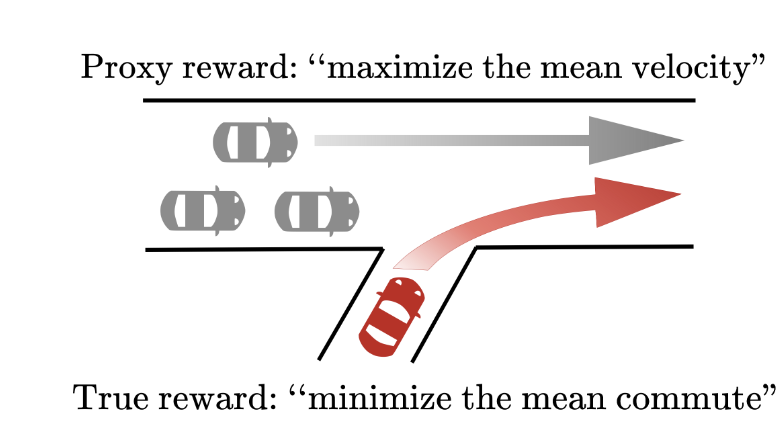
\includegraphics[width=3in]{commute_time.png}
    \caption{Pan, Bhatia, Steinhardt ICLR 2022; \url{https://openreview.net/pdf?id=JYtwGwIL7ye}}
    \label{fig:commute}
\end{figure}
\begin{enumerate}[label=(\alph*)]
    \item  Explain why the optimal policy for the AI car is not to merge onto the highway. [2 pts]
    \item Note this behavior is not aligned with the true reward function. Share some ideas about alternate reward functions (that are not minimizing commute) that might still be easier to optimize, but would not result in the AI car never merging. Your answer should be 2-5 sentences and can include equations: there is not a single answer and reasonable solutions will be given full credit. [3 pts]

\end{enumerate}



% \begin{tcolorbox}[breakable]
% \end{tcolorbox}

\newpage

\section{Bellman Residuals and performance bounds [30 pts]}

In this problem, we will study value functions and properties of the Bellman backup operator.
\\

\noindent \textbf{Definitions:} \noindent Recall that a value function is a $|S|$-dimensional vector where $|S|$ is the number of states of the MDP. When we use the term $V$ in these expressions as an ``arbitrary value function'', we mean that $V$ is an arbitrary $|S|$-dimensional vector which need not be aligned with the definition of the MDP at all. 
On the other hand, $V^\pi$ is a value function that is achieved by some policy $\pi$ in the MDP.
For example, say the MDP has 2 states and only negative immediate rewards. $V = [1,1]$ would be a valid choice for $V$ even though this value function can never be achieved by any policy $\pi$, but we can never have a $V^\pi = [1,1]$. This distinction between $V$ and $V^\pi$ is important for this question and more broadly in reinforcement learning.
\\


\noindent \textbf{Properties of Bellman Operators:} In the first part of this problem, we will explore some general and useful properties of the Bellman backup operator, which was introduced during lecture. We know that the Bellman backup operator $B$, defined below is a contraction with the fixed point as $V^*$, the optimal value function of the MDP. The symbols have their usual meanings. $\gamma$ is the discount factor and $0 \leq \gamma < 1$. In all parts, $\|v\| = \max_{s} | v(s) |$ is the infinity norm of the vector.

\begin{equation}
    (BV)(s) = \max_a r(s, a) + \gamma\sum_{s' \in S}p(s'|s,a)V(s')
\end{equation}

\noindent We also saw the contraction operator $B^\pi$ with the fixed point $V^\pi$, which is the Bellman backup operator for a particular policy given below:

\begin{equation}
    (B^\pi V)(s) = r(s,\pi(s)) + \gamma\sum_{s' \in S}p(s'|s,\pi(s))V(s')
\end{equation}


\noindent In this case, we'll assume $\pi$ is deterministic, but it doesn't have to be in general. In class, we showed that $|| BV - BV' || \leq \gamma ||V - V'||$ for two arbitrary value functions $V$ and $V'$. 

\begin{enumerate}[label=(\alph*)]
    \item Show that the analogous inequality, $|| B^\pi V - B^\pi V' || \leq \gamma ||V - V'||$, also holds. [3 pts].
    
    \item Prove that the fixed point for $B^\pi$ is unique. Recall that the fixed point is defined as $V$ satisfying $V = B^\pi V$. You may assume that a fixed point exists. \textit{Hint:} Consider proof by contradiction. [3 pts].
    
    \item Suppose that $V$ and $V'$ are vectors satisfying $V(s) \leq V'(s)$ for all $s$. Show that $B^\pi V(s) \leq B^\pi V'(s)$ for all $s$. Note that all of these inequalities are elementwise. [3 pts].


\end{enumerate}




\noindent \textbf{Bellman Residuals:} Having gained some intuition for value functions and the Bellman operators, we now turn to understanding how policies can be extracted and what their performance might look like. We can extract a greedy policy $\pi$ from an arbitrary value function $V$ using the equation below. 
\begin{equation}
    \pi(s) = \argmax_{a} [{r(s,a) + \gamma\sum_{s' \in S}p(s'|s,a)V(s')}]
\end{equation}

It is often helpful to know what the performance will be if we extract a greedy policy from an arbitrary value function. To see this, we introduce the notion of a Bellman residual.

Define the Bellman residual to be $(BV - V)$ and the Bellman error magnitude to be $||BV - V||$.

\begin{enumerate}
    \item[(d)] For what value function $V$ does the Bellman error magnitude $\|BV - V \|$ equal 0? Why? [2 pts]
    \item[(e)] Prove the following statements for an arbitrary value function $V$ and any policy $\pi$.  [5 pts]\\
    \textit{Hint:} Try leveraging the triangle inequality by inserting a zero term.
    \begin{equation}
        ||V - V^\pi|| \leq \frac{||V - B^\pi V||}{1-\gamma}
    \end{equation}
    \begin{equation}
        ||V - V^*|| \leq \frac{||V - BV||}{1-\gamma}
    \end{equation}
\end{enumerate}

\noindent The result you proved in part (e) will be useful in proving a bound on the policy performance in the next few parts. Given the Bellman residual, we will now try to derive a bound on the policy performance, $V^\pi$.

\begin{enumerate}
    \item[(f)] Let $V$ be an arbitrary value function and $\pi$ be the greedy policy extracted from $V$. Let $\epsilon = ||BV-V||$ be the Bellman error magnitude for $V$. Prove the following for any state $s$. [5 pts]\\
    \textit{Hint:} Try to use the results from part (e).
    \begin{equation}
        V^\pi(s) \geq V^*(s) - \frac{2\epsilon}{1-\gamma}
    \end{equation}
        \item[(g)] Give an example real-world application or domain where having a lower bound on $V^\pi(s)$ would be useful. [2 pt]

    \item[(h)] Suppose we have another value function $V'$ and extract its greedy policy $\pi'$.  $\|B V' - V' \| = \epsilon = \|B V - V\|$. Does the above lower bound imply that $V^\pi(s) = V^{\pi'}(s)$ at any $s$? [2 pts]

\end{enumerate}

\noindent {A little bit more notation:} define $V \leq V'$ if $\forall s$, $V(s) \leq V'(s)$. 
\\



\noindent What if our algorithm returns a $V$ that satisfies $V^* \leq V$? I.e., it returns a value function that is better than the optimal value function of the MDP. Once again, remember that $V$ can be any vector, not necessarily achievable in the MDP but we would still like to bound the performance of $V^\pi$ where $\pi$ is extracted from said $V$. We will show that if this condition is met, then we can achieve an even tighter bound on policy performance.



\begin{enumerate}
    \item[(i)] Using the same notation and setup as part (e), if $V^* \leq V$, show the following holds for any state $s$. [5 pts]\\
    \textit{Hint:} Recall that $\forall \pi$, $V^\pi \leq V^*$. (why?)
    \begin{equation}
        V^\pi(s) \geq V^*(s) - \frac{\epsilon}{1-\gamma}
    \end{equation}
\end{enumerate}

\noindent \textbf{Intuition:} A useful way to interpret the results from parts (h) (and (i)) is based on the observation that a constant immediate reward of $r$ at every time-step leads to an overall discounted reward of $r + \gamma r + \gamma^2 r + \ldots = \frac{r}{1-\gamma}$. Thus, the above results say that a state value function $V$ with Bellman error magnitude $\epsilon$ yields a greedy policy whose reward per step (on average), differs from optimal by at most $2\epsilon$. So, if we develop an algorithm that reduces the Bellman residual, we're also able to bound the performance of the policy extracted from the value function outputted by that algorithm, which is very useful!
\\

\noindent \textbf{Challenges:} Try to prove the following if you're interested. \textbf{These parts will not be graded.}

\begin{enumerate}
    \item[(j)] It's not easy to show that the condition $V^* \leq V$ holds because we often don't know $V^*$ of the MDP. Show that if $BV \leq V$ then $V^* \leq V$. Note that this sufficient condition is much easier to check and does not require knowledge of $V^*$. \\
    \textit{Hint}: Try to apply induction. What is $\lim\limits_{n \rightarrow \infty} B^n V$?

\item[(k)] It is possible to make the bounds from parts (i) and (j) tighter. 
Let $V$ be an arbitrary value function and $\pi$ be the greedy policy extracted from $V$. Let $\epsilon = ||BV-V||$ be the Bellman error magnitude for $V$. Prove the following for any state $s$:
\begin{equation}
        V^\pi(s) \geq V^*(s) - \frac{2\gamma\epsilon}{1-\gamma}
\end{equation}
Further, if $V^* \leq V$, prove for any state $s$
\begin{equation}
        V^\pi(s) \geq V^*(s) - \frac{\gamma\epsilon}{1-\gamma}
\end{equation}
\end{enumerate}






\noindent 


% \begin{tcolorbox}[breakable]
% \end{tcolorbox}


\newpage

\section{RiverSwim MDP [25 pts]}
Now you will implement value iteration and policy iteration for the RiverSwim environment (see picture below\footnote{Figure copied from \href{https://proceedings.neurips.cc/paper/2013/hash/6a5889bb0190d0211a991f47bb19a777-Abstract.html}{(Osband \& Van Roy, 2013)}.}) of \href{https://www.sciencedirect.com/science/article/pii/S0022000008000767}{(Strehl \& Littman, 2008)}.
\begin{figure}[h]
    \centering
    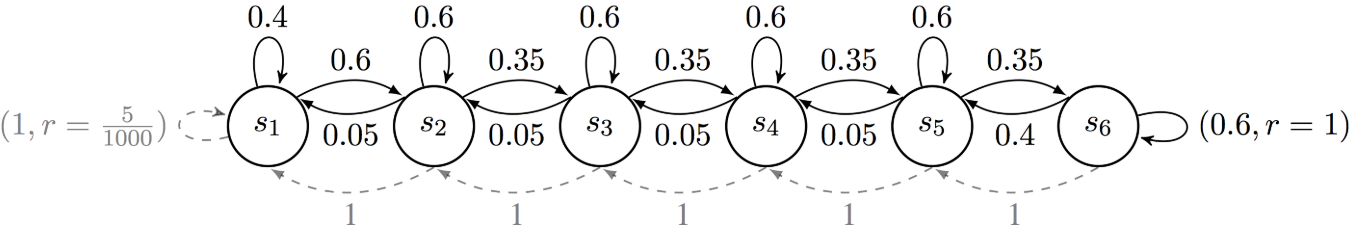
\includegraphics[width=\linewidth]{RiverSwim.png}
    \caption{The RiverSwim MDP where dashed and solid arrows represent transitions for the \textsc{LEFT} and \textsc{RIGHT} actions, respectively. The assignment uses a modified, customizable version of what is shown above where there are three different strengths (\textsc{WEAK}, \textsc{MEDIUM}, or \textsc{STRONG}) of the current (transition probabilities for being pushed back or successfully swimming \textsc{RIGHT}).}
    \label{fig:riverswim}
\end{figure}

\noindent \textbf{Setup:} This assignment needs to be completed with Python3 and \texttt{numpy}. 
% We have provided a \texttt{requirements.txt} file that contains all the associated Python libraries you will need to complete this assignment. You can go through the file and install all the libraries by running \texttt{pip install -r requirements.txt} in the terminal. We highly recommend that you do this in a \href{https://docs.python.org/3/library/venv.html}{virtual environment} dedicated for this assignment to avoid any dependency conflicts. 
% \textbf{While programming, please ignore any \texttt{DeprecationWarning} you may see}.
\\

\noindent \textbf{Submission:} There is a \texttt{Makefile} provided that will help you submit the assignment. Please run \texttt{make clean} followed by \texttt{make submit} in the terminal and submit the resulting zip file on Gradescope.


\begin{enumerate}[label=(\alph*)]
\item \textbf{(coding)} Read through \texttt{vi\_and\_pi.py} and implement \texttt{bellman\_backup}. Return the value associated with a single Bellman backup performed for an input state-action pair. [4 pts]\\


\item \textbf{(coding)} Implement \texttt{policy\_evaluation}, \texttt{policy\_improvement} and \texttt{policy\_iteration} in  \texttt{vi\_and\_pi.py}. Return the optimal value function and the optimal policy. [8pts]\\


\item \textbf{(coding)} Implement \texttt{value\_iteration} in \texttt{vi\_and\_pi.py}. Return the optimal value function and the optimal policy. [8 pts]\\


\item \textbf{(written)} Run both methods on RiverSwim with a \textsc{weak} current strength and find the largest discount factor (\textbf{only} up to two decimal places) such that an optimal agent starting in the initial far-left state (state $s_1$ in Figure \ref{fig:riverswim}) \textbf{does not} swim up the river (that is, does not go \textsc{RIGHT}). Using the value you find, interpret why this behavior makes sense. Now repeat this for RiverSwim with \textsc{medium} and \textsc{strong} currents, respectively. Describe and explain the changes in optimal values and discount factors you obtain both quantitatively and qualitatively. [5 pts]\\ \\
\textit{Sanity Check:} For RiverSwim with a discount factor $\gamma = 0.99$ and a \textsc{weak} current, the values for the left-most and right-most states ($s_1$ and $s_6$ in Figure \ref{fig:riverswim} above) are \texttt{30.328} and \texttt{36.859}. The value functions from VI and PI should be within error tolerance $10^{-3}$ of these values. You can use this to verify your implementation. For grading purposes, we shall test your implementation against other hidden test cases as well.

\end{enumerate}


% \begin{tcolorbox}[breakable]
% \end{tcolorbox}



\end{document} 